\documentclass{article}
\usepackage[ruled,vlined,linesnumbered]{algorithm2e}
\usepackage{algpseudocode}
\usepackage{amsmath}
\usepackage{amsthm}
\usepackage{graphicx}
\usepackage{subfigure}
\usepackage{float}
\usepackage{amsmath }
\usepackage{amsfonts }
\usepackage{pdfpages}
\usepackage{epsfig}
\usepackage{graphicx}
\usepackage{arydshln}
\usepackage{verbatim}
\usepackage{subfigure}
\usepackage{enumerate}
\usepackage{rotating}
\usepackage{threeparttable}
\usepackage{caption}
\usepackage{epsfig}
\usepackage{cite}
\usepackage{times}
\usepackage{geometry}
\usepackage{tikz}
\geometry{a4paper}
\renewcommand{\baselinestretch}{1.5}
\usepackage[colorlinks,linkcolor=blue]{hyperref}
\begin{document}
\title{AI3602 Data Mining Homework 5}
\author{Kailing Wang 521030910356}
\date{June 1.2024}
\maketitle

\section*{Question 1}

(1)
To achieve $\epsilon-$diffrential privacy, we choose the scale parameter b as
\begin{equation}
	b = \frac{\Delta f}{\epsilon},
\end{equation}
where
\begin{equation}
	\Delta f = \max_{|D_1 \Delta D_2| = 1} \| f(D_1) - f(D_2) \|_1.
\end{equation}
Oh, here given L1 sensitivity, is 1 so $b = \frac{1}{\epsilon}$.

\noindent(2)
\begin{equation}
	\sigma = \frac{\Delta f \sqrt{2\ln(1.25/\delta)}}{\epsilon}
\end{equation}
where
\begin{equation}
	\Delta f = \max_{|D_1 \Delta D_2| = 1} \| f(D_1) - f(D_2) \|_2.
\end{equation}
So $\sigma = \frac{\sqrt{2\ln(1.25/\delta)}}{\epsilon}$. Note that I assume the $\sigma$ in the question should be $\sigma^2$ as normal representation.

\section*{Question 2}

To satisfy \(\epsilon\)-differential privacy, the following condition must hold:
\begin{align}
e^\epsilon &\geq \frac{p}{\frac{1 - p}{m - 1}} \\
e^\epsilon (1 - p) &\geq p (m - 1) \\
e^\epsilon - e^\epsilon p &\geq p (m - 1) \\
e^\epsilon &\geq p (m - 1 + e^\epsilon)
\end{align}

Thus, the probability \(p\) that satisfies \(\epsilon\)-differential privacy is:
\begin{equation}
p \leq \frac{e^\epsilon}{(m - 1) + e^\epsilon}
\end{equation}

To satisfy \(\epsilon\)-differential privacy when \(y\) is not the correct answer, the following condition must hold:
\begin{align}
e^\epsilon &\geq \frac{\frac{1 - p}{m - 1}}{p} \\
e^\epsilon p &\geq \frac{1 - p}{m - 1} \\
e^\epsilon p (m - 1) &\geq 1 - p \\
e^\epsilon p (m - 1) + p &\geq 1 \\
p (e^\epsilon (m - 1) + 1) &\geq 1
\end{align}

Thus, the probability \(p\) that satisfies \(\epsilon\)-differential privacy is:
\begin{equation}
p \geq \frac{1}{(m - 1) e^\epsilon + 1}
\end{equation}

Combining both conditions, the probability \(p\) must satisfy:
\begin{equation}
\frac{1}{(m - 1) e^\epsilon + 1} \leq p \leq \frac{e^\epsilon}{(m - 1) + e^\epsilon}
\end{equation}

\section*{Original Questions}
\begin{figure}[h!]
	\centering
	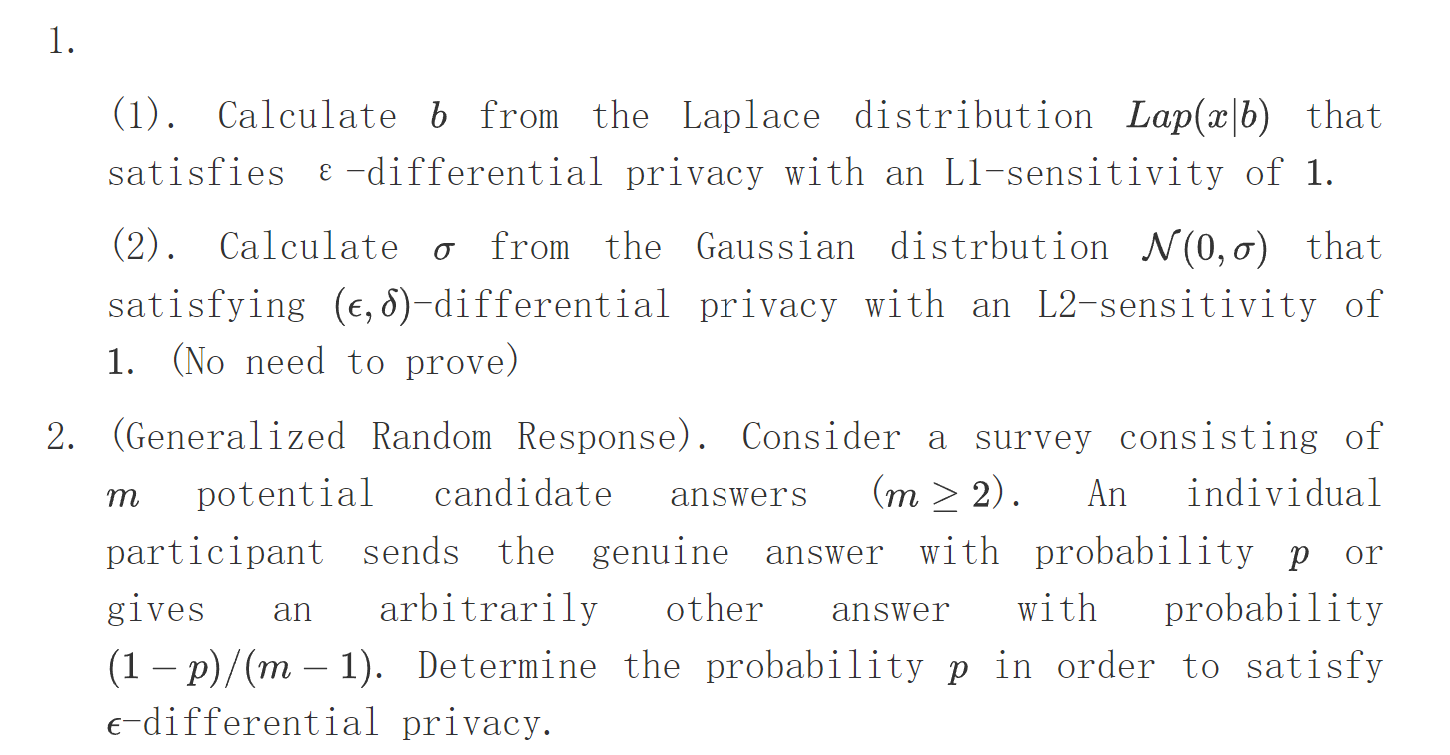
\includegraphics[width=1\textwidth]{hw5.png}
	\caption{Question 1}
	\label{fig:1}
\end{figure}
\section*{Reference}
\href{https://www.cis.upenn.edu/~aaroth/chatgpt_lecture_notes.pdf}{lecture notes}
\end{document}
